\section{Runtime Libraries}\label{sec:runtime}

%-----------------------------------------------------------------------------
\subsection{Layered Communication Libraries}
%-----------------------------------------------------------------------------

3種:one sided, collective, atomic. このうちcollectiveとatomicはMPIの機能をそのまま使う。それ以上の工夫はない。one sidedはallocate/freeとput/getと同期。lower-level通信層のバリエーションを吸収するライブラリ層を設けた。階層の図。

\begin{figure}[tbh]
  \begin{center}
  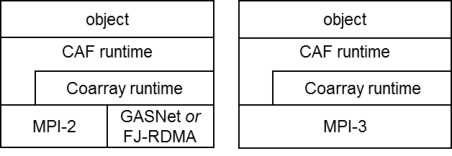
\includegraphics[scale=1.0]{figs/layer.pdf}
  \caption{Layered Communicaion Libraries(左の絵だけでよい)}\label{fig:layer}
  \end{center}
\end{figure}

cf.\ air:/Users/iwashita/Desktop/coarray/Project\_Coarray/coarray implement 6-1.docx 他


To implement one-sided communication, the XcalableMP (XMP) runtime library selects one of the 
{\em communication libraries}, MPI-3, GASNet, or Fujitsu’s native interface FJ-RDMA, 
as specified at build time. All coarray data must be {\em registered} to the communication 
library to be referenced or defined via the communication library.

MPI-3 can be selected for all platform on which MPI-3 is implemented. Coarrays are 
registered and deregistered at the start and end point of the MPI window. 
Coarrays are performed one-sided communication by {\tt MPI\_Put} and {\tt MPI\_Get}, 
and synchronized by {\tt MPI\_Win\_fence}. 
Implementation on MPI incurs certain costs for dynamic allocation of coarrays and 
waiting for communication completion.

GASNet can be selected for more advanced implementation over InfiniBand. 
Since allocation and registration of are inseparable and can be done only once 
on GASNet, the implementation allocates and registers a huge pool at the startup 
of program execution to contain all coarray variables. 
The XMP runtime should allocate and deallocate coarrays not using the Fortran 
library but using the memory manager made for the pool.

FJ-RDMA can be selected for the implementation over Tofu interconnect of the K computer 
and Fujitsu PRIMEHPC FX10 and FX100. Basically, each coarray is allocated by the Fortran 
library and registered with {\tt FJMPI\_Rdma\_reg\_mem}. And it is deregistered with 
{\tt FJMPI\_Rdma\_dereg\_mem} before deallocated by the Fortran library. 
One-sided communication is performed with {\tt FJMPI\_Rdma\_put} and {\tt FJMPI\_Rdma\_get}, 
which include confirmation of communication completion.


\subsection{Intermediate Communication Library Interface}


次元の概念とcontiguityを上位層で解決するため結果的に必要なインタフェースは少なくなった。表

\begin{table}
 \begin{center}
  \caption{使用したCoarrayランタイムインタフェース(未公開機能関連を除く)}
  \begin{tabular}{|l|l|}
\hline
割付け・解放と登録
& 1. \verb|_XMP_coarray_malloc_image_info_1|\\
& 2. \verb|_XMP_coarray_malloc_info_1|\\
& 3. \verb|_XMP_coarray_malloc_do|\\
& 4. \verb|_XMP_coarray_regmem_do|\\
& 5. \verb|_XMP_coarray_lastly_deallocate|\\
\hline
片側通信
& 6. \verb|_XMP_coarray_shortcut_get|\\
& 7. \verb|_XMP_coarray_shortcut_put|\\
\hline
同期
& 8. \verb|xmp_sync_all|\\
& 9. \verb|xmp_sync_image|\\
& 10 \verb|.xmp_sync_images|\\
& 11 \verb|.xmp_sync_images_all|\\
& 12 \verb|.xmp_sync_memory|\\
\hline
atomic通信
& 13 \verb|._XMP_atomic_define_0|\\
& 14 \verb|._XMP_atomic_define_1|\\
& 15 \verb|._XMP_atomic_ref_0|\\
& 16 \verb|._XMP_atomic_ref_1|\\
\hline
問合せ
& 17 \verb|.xmp_all_num_nodes|\\
\hline
エラー処理
& 18 \verb|._XMP_fatal|\\
\hline
  \end{tabular}
 \end{center}
\end{table}


下位通信層は通信ライブラリを隠蔽する。例えばregisterは

しかしあらわになるものがあってオブジェクトが通信ライブラリを意識するモードで分ける。

